\section{Validación experimental}

\paragraph{Método.} \texttt{Informe/code/experimentos.py} genera instancias sintéticas (semilla 2026)
de 6 tamaños crecientes por experimento, duplicando el tamaño en cada paso. Cada punto es la
mediana de 7 mediciones con \texttt{time.perf\_counter}, tras una ejecución de calentamiento que no
se mide y con el recolector de basura apagado. Luego se ajusta $t\approx c\cdot T(n)$ por mínimos
cuadrados: si la deducción es correcta, el ajuste es casi perfecto ($R^2\approx1$) y el cociente
$t/T(n)$ se mantiene casi constante. Los datos están en \texttt{Informe/code/experimentos.csv}.

\begin{center}
\begin{tabularx}{\linewidth}{>{\raggedright}Xlccc}
\cabecera \cab{Experimento} & \cab{$T(n)$ teórico} & \cab{$c$ (s)} & \cab{$R^2$} & \cab{Crecimiento} \\
Reparto, $N=2000$, $B$ de $2\cdot10^4$ a $6.4\cdot10^5$ & $N+B\ln N$ & $7.5\cdot10^{-8}$ & 0.9992 & $B\times32\to t\times29.5$ \\
Reparto, $B=20N$, $N$ de 2000 a 64\,000 & $N+20N\ln N$ & $1.6\cdot10^{-7}$ & 0.9859 & $N\times32\to t\times89$ \\
Selección, $k=20$, $N$ de 1000 a 32\,000 & $Nk$ & $1.3\cdot10^{-7}$ & 0.9997 & $N\times32\to t\times32.6$ \\
Selección, $N=8000$, $k$ de 5 a 160 & $Nk$ & $1.7\cdot10^{-7}$ & 0.9988 & $k\times32\to t\times40.5$ \\
\bottomrule
\end{tabularx}
\end{center}

\begin{figure}[H]
  \centering
  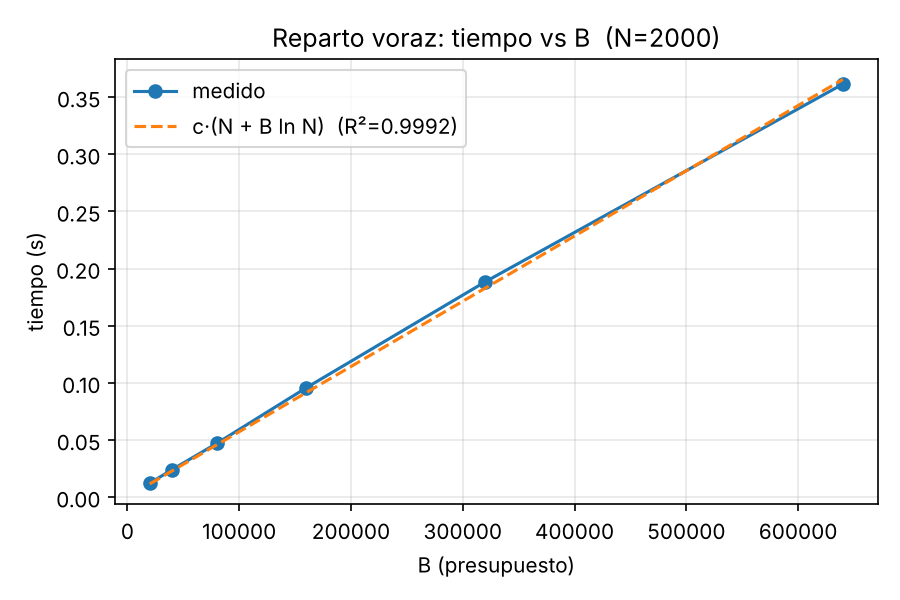
\includegraphics[width=0.49\linewidth]{img/reparto_vs_B.png}\hfill
  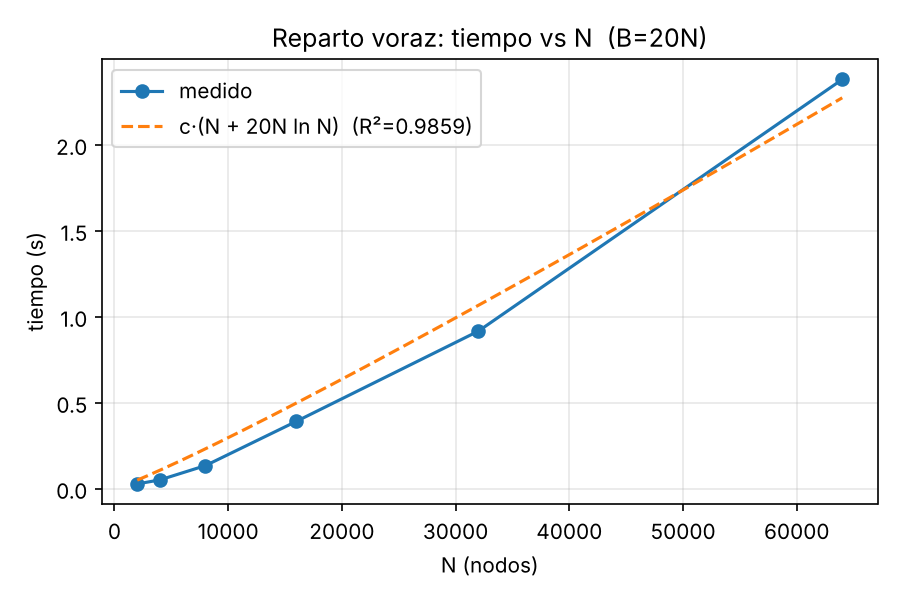
\includegraphics[width=0.49\linewidth]{img/reparto_vs_N.png}
  \caption{Reparto voraz: tiempo medido (puntos) frente a $c\cdot T(n)$ ajustado (línea).}
\end{figure}

\begin{figure}[H]
  \centering
  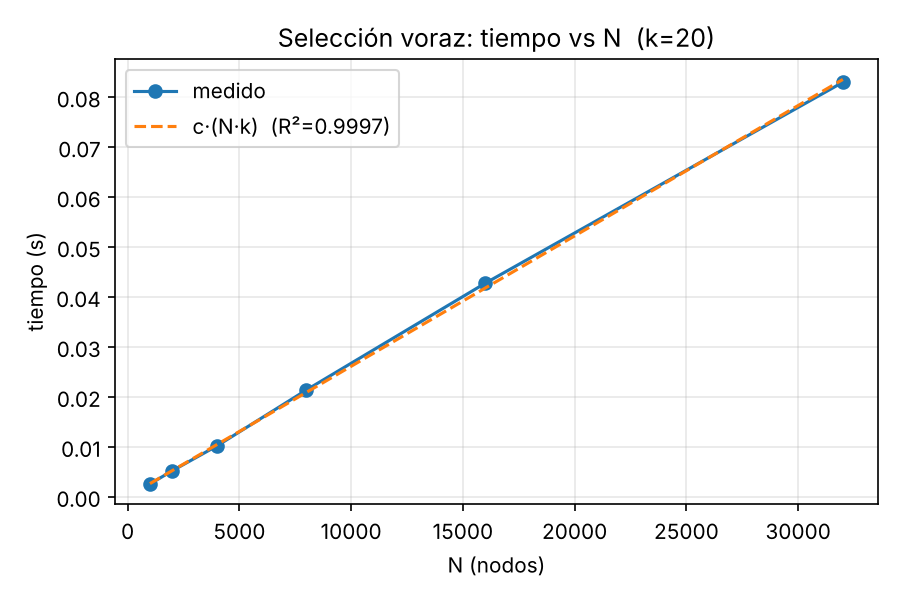
\includegraphics[width=0.49\linewidth]{img/seleccion_vs_N.png}\hfill
  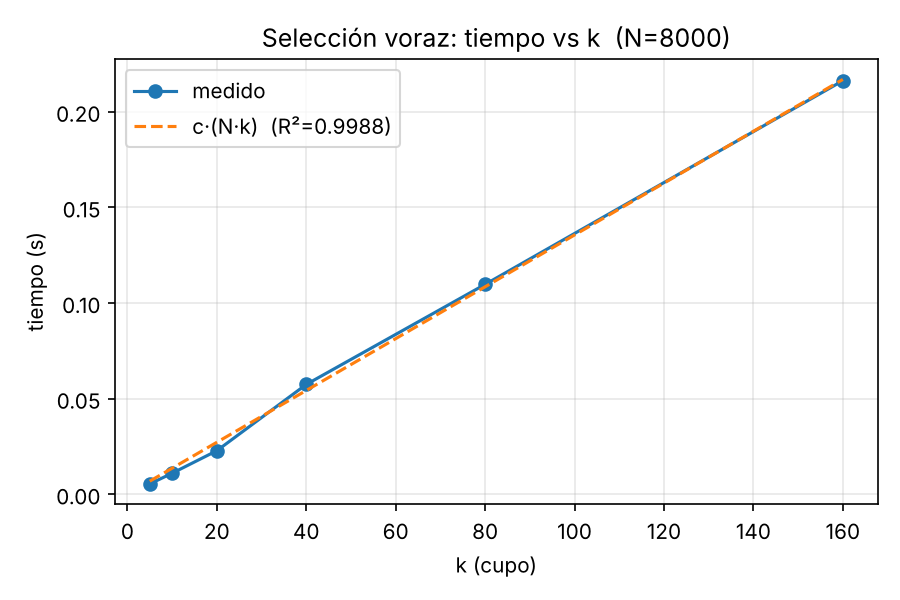
\includegraphics[width=0.49\linewidth]{img/seleccion_vs_k.png}
  \caption{Selección voraz: tiempo medido frente a $c\cdot Nk$ ajustado.}
\end{figure}

\paragraph{Análisis.}
\begin{itemize}
  \item \textbf{Reparto contra $B$:} el tiempo es lineal en $B$ ($\times29.5$ para $B\times32$;
  el cociente $t/T$ pasa de $7.9\cdot10^{-8}$ a $7.4\cdot10^{-8}$), como predice el término $B\log N$.
  \item \textbf{Selección:} lineal en $N$ y en $k$ ($R^2\ge0.998$), con el desempate por peso
  incluido. El número de evaluaciones es exactamente $kN-k(k-1)/2$, comprobado por una prueba
  automática. Contra $N$ el cociente $t/T$ se mantiene entre $1.27$ y $1.34\cdot10^{-7}$
  ($\times32.6$). Contra $k$ crece algo más que $\times32$ ($\times40.5$; el cociente sube de
  $1.33$ a $1.69\cdot10^{-7}$), por costos de memoria al recorrer listas más largas en cada paso;
  el orden de crecimiento no cambia.
  \item \textbf{Reparto contra $N$:} crece más que el modelo ($\times89$ frente a $\times46$ teórico). No es
  el algoritmo: \texttt{Informe/code/diagnostico\_heap.py} mide con $B$ fijo el costo por unidad,
  y de $N=2000$ a $64\,000$ el reparto crece $\times3.73$ y \texttt{heapq.heapreplace} aislado
  $\times3.68$, frente a $\times1.46$ esperado por $\log N$. El exceso está en el montículo de
  Python. Es coherente con que el análisis usa el modelo RAM (todo acceso cuesta lo mismo) y un
  montículo grande ya no cabe en la caché del procesador; esa causa física no se midió
  directamente. El crecimiento sigue muy lejos de uno cuadrático ($\times1024$).
\end{itemize}

\paragraph{Exacto frente a voraz.} Con $N=40$ y $k=20$, el exacto necesitaría
$\binom{40}{20}\approx1.4\cdot10^{11}$ evaluaciones (días de cómputo), mientras que el voraz
resuelve $N=32\,000$ con $k=20$ en unos 0.08 s.
